
%%% Local Variables:
%%% mode: latex
%%% TeX-master: "main"
%%% End:

\chapter{Geometrical Optics}

\section{Refraction at a Spherical Interface}

\begin{figure}[H]
  \centering
  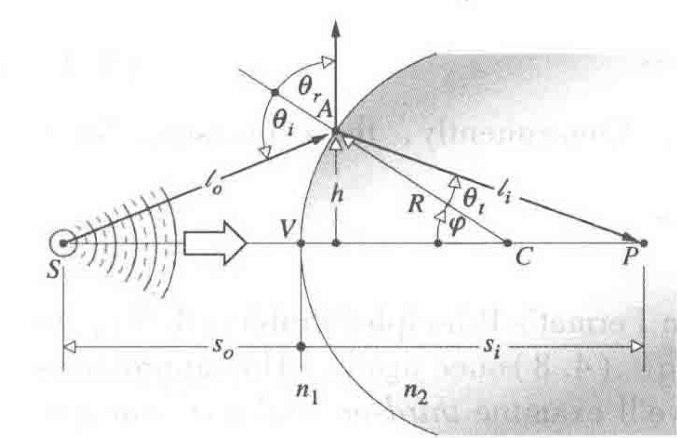
\includegraphics[width=0.4\linewidth]{figures/Refraction at a Spherical Interface}
  \label{fig:}
\end{figure}

\begin{equation*}
  \begin{aligned}
    \dfrac{n_1}{s_o} + \dfrac{n_2}{s_i} = \dfrac{n_2 - n_1}{R}   
  \end{aligned}
\end{equation*}

Let $s_i = \infty$, the object focus

\begin{equation*}
  \begin{aligned}
    f_0 = \dfrac{n_1}{n_2 - n_1} R 
  \end{aligned}
\end{equation*}

Let $s_o = \infty$, the image focus

\begin{equation*}
  \begin{aligned}
    f_i = \dfrac{n_2}{n_2 - n_1} R 
  \end{aligned}
\end{equation*}

\begin{figure}[H]
  \centering
  \begin{subfigure}{.3\textwidth}
    \centering
    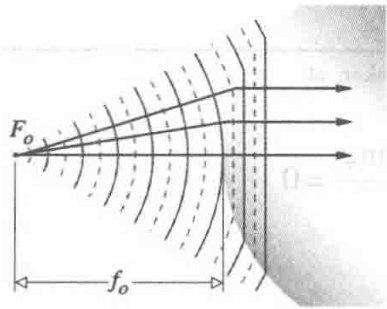
\includegraphics[width=\linewidth]{figures/Refraction at a Spherical Interface 1.jpg}
    \label{fig:}
  \end{subfigure}
  \hspace{2cm}
  \begin{subfigure}{.4\textwidth}
    \centering
    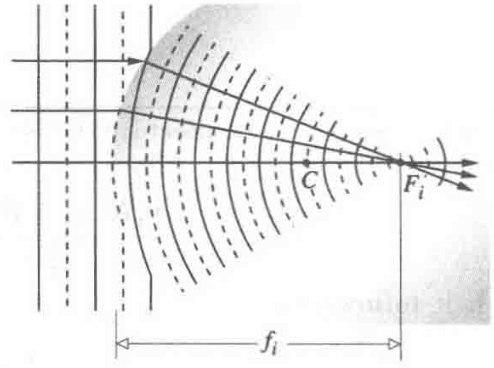
\includegraphics[width=\linewidth]{figures/Refraction at a Spherical Interface 2.jpg}
    \label{fig:}
  \end{subfigure}
  \label{fig:}
\end{figure}


\section{Lenses}

\begin{figure}[H]
  \centering
  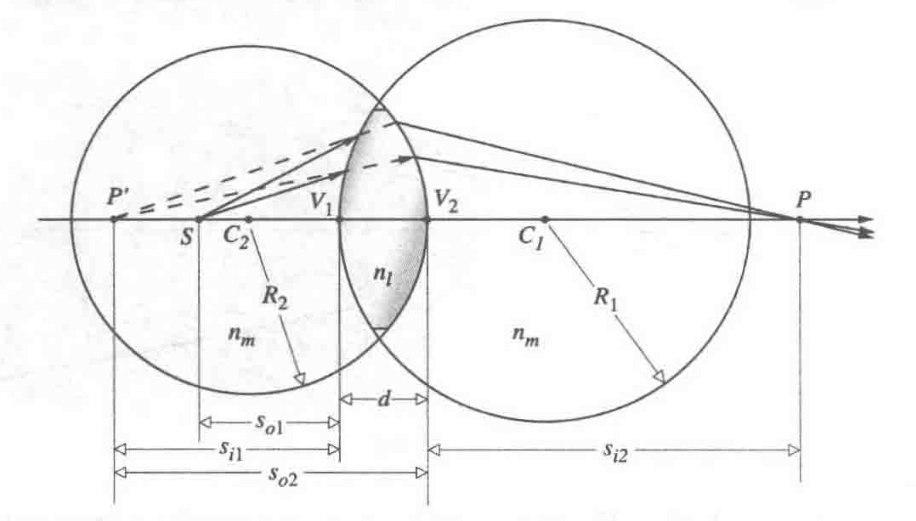
\includegraphics[width=0.5\linewidth]{figures/Thin-Lens.jpg}
  \label{fig:}
\end{figure}

\begin{equation*}
  \begin{aligned}
    \dfrac{n_m}{s_{o1}} + \dfrac{n_m}{s_{i2}} = \left( n_l - n_m \right) \left( \dfrac{1}{R_1} - \dfrac{1}{R_2}   \right) + \dfrac{n_l d}{\left( s_{i1} - d \right) s_{i1}} 
  \end{aligned}
\end{equation*}

For lenses in the air, where $n_m = 1$

\begin{equation*}
  \begin{aligned}
    \dfrac{1}{s_{o1}} + \dfrac{1}{s_{i2}} = \left( n_l - 1 \right) \left( \dfrac{1}{R_1} - \dfrac{1}{R_2}   \right) + \dfrac{n_l d}{\left( s_{i1} - d \right) s_{i1}} 
  \end{aligned}
\end{equation*}

For thin lenses, $d \approx 0$

\begin{equation*}
  \begin{aligned}
    \dfrac{1}{s_{o1}} + \dfrac{1}{s_{i2}} = \left( n_l - 1 \right) \left( \dfrac{1}{R_1} - \dfrac{1}{R_2}   \right) = \dfrac{1}{f} 
  \end{aligned}
\end{equation*}

Which is the Gaussian Lens Formula.

\section{Magnification}

\begin{figure}[H]
  \centering
  \begin{subfigure}{.5\textwidth}
    \centering
      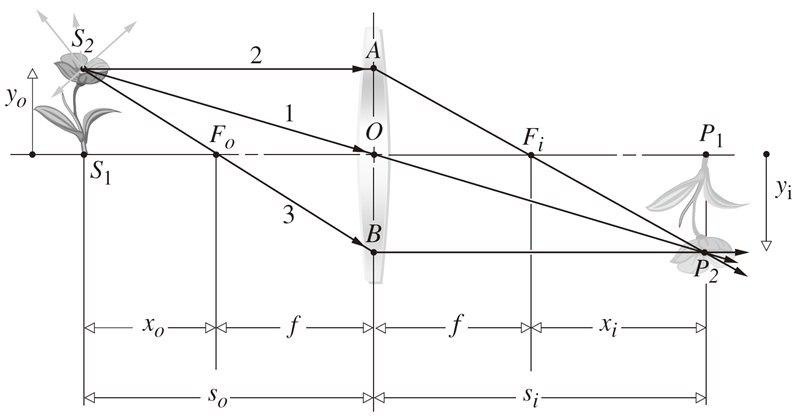
\includegraphics[width=\linewidth]{figures/Magnification transverse.jpg}
    \label{fig:}
  \end{subfigure}%
  \begin{subfigure}{.5\textwidth}
    \centering
      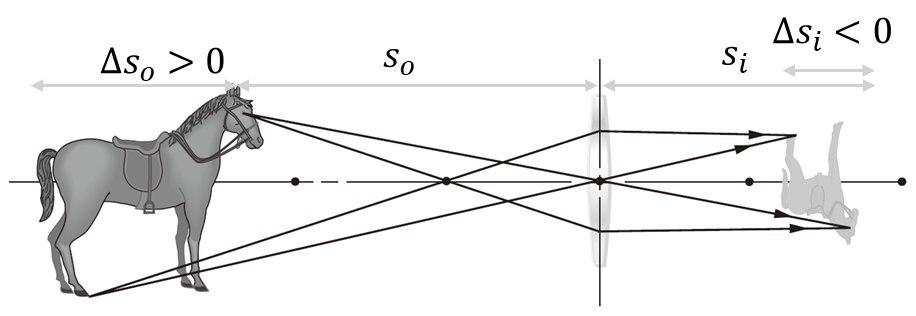
\includegraphics[width=\linewidth]{figures/Magnification longitudinal.jpg}
    \label{fig:}
  \end{subfigure}
  \label{fig:}
\end{figure}


\begin{equation*}
  \left\{
  \begin{aligned}
    \dfrac{y_o}{|y_i|} = \dfrac{f}{x_i} \\
    \dfrac{|y_i|}{y_o} = \dfrac{f}{x_o}  
  \end{aligned}
  \right.
\end{equation*}

Newton's formula

\begin{equation*}
  \begin{aligned}
    x_o x_i = f^2
  \end{aligned}
\end{equation*}


Transverse Magnification

\begin{equation*}
  \begin{aligned}
    M_T = \dfrac{y_i}{|y_o|} = - \dfrac{s_o}{s_i} = - \dfrac{f}{x_o} = - \dfrac{x_i}{f}  
  \end{aligned}
\end{equation*}

Longitudinal Magnification

\begin{equation*}
  \begin{aligned}
    M_L = \dfrac{\md x_i}{\md x_o} = \dfrac{\md}{\md x_o} \left( \dfrac{f^2}{x_o}  \right) = - \dfrac{f^2}{x_o^2} = - M_T^2   
  \end{aligned}
\end{equation*}

\section{Prism}

\begin{figure}[H]
  \centering
  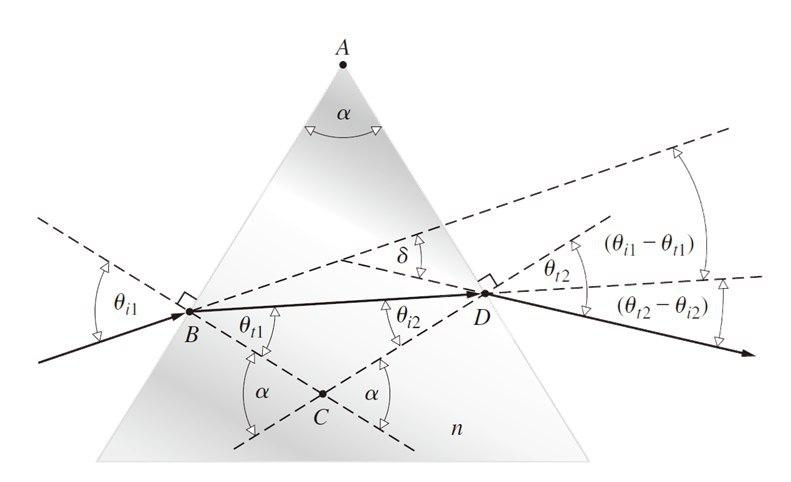
\includegraphics[width=0.5\linewidth]{figures/Prism}
  \label{fig:}
\end{figure}

\begin{equation*}
  \left\{
  \begin{aligned}
    \delta &= \left( \theta_{i1} - \theta_{t1} \right) + \left( \theta_{t2} - \theta_{i2} \right) \\
    \alpha &= \theta_{t1} + \theta_{i2}
  \end{aligned}
  \right.
\end{equation*}

\begin{equation*}
  \begin{aligned}
    \delta &= \theta_{i1} + \theta_{t2} - \alpha
  \end{aligned}
\end{equation*}

\begin{equation*}
  \begin{aligned}
    \theta_{t2} &= \arcsin \left( n \sin \theta_{i2} \right) = \arcsin \left[ n \sin \left( \alpha - \theta_{t1} \right) \right] = \arcsin \left[ n \left( \sin \alpha \cos \theta_{t1} - \cos \alpha \sin \theta_{t1} \right) \right] \\
    &= \arcsin \left[ n \left( \sin \alpha \sqrt{1 - \sin^2 \theta_{t1}} - \cos \alpha \sin \theta_{t1} \right) \right] \\
    &= \arcsin \left[ n \left( \sin \alpha \sqrt{1 - n^2 \sin^2 \theta_{i1}} - \cos \alpha \sin \theta_{t1} \right) \right] \\
    \delta &= \theta_{i1} + \arcsin \left[ n \left( \sin \alpha \sqrt{1 - n^2 \sin^2 \theta_{i1}} - \cos \alpha \sin \theta_{t1} \right) \right] - \alpha
  \end{aligned}
\end{equation*}


